
\chapter{GCSE Transformation Questions}
\begin{enumerate}
  \item \mbox{}
  \begin{figure}[H]
    \centering
    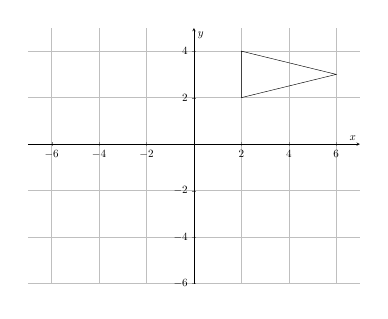
\begin{tikzpicture}[scale = 0.4]
      \begin{axis}[
          xmin = -7, xmax = 7,
          ymin = -6, ymax = 5,
          grid = both,
          axis lines = middle,
          width = \textwidth,
          height = 0.8\textwidth,
          xlabel = {$x$},
          ylabel = {$y$},
        ]
        \draw (2,2) -- (2,4) -- (6,3) -- (2,2);
      \end{axis}
    \end{tikzpicture}
  \end{figure}
  On the grid, enlarge the triangle by scale factor $-\frac{1}{2}$, centre $(0, -2)$.\mrk{2}
  \item \mbox{}
  \begin{figure}[H]
    \centering
    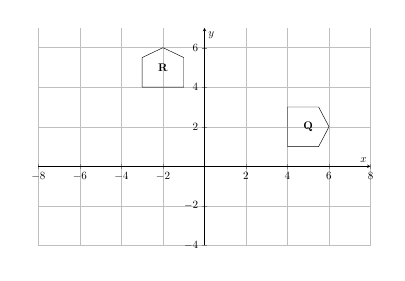
\begin{tikzpicture}[scale = 0.4]
      \begin{axis}[
          xmin = -8, xmax = 8,
          ymin = -4, ymax = 7,
          grid = both,
          axis lines = middle,
          width = \textwidth,
          height = 0.7\textwidth,
          xlabel = {$x$},
          ylabel = {$y$},
        ]
        \draw (-3,4) -- (-3,5.5) -- (-2,6) -- (-1,5.5) -- (-1,4) -- (-3,4);
        \draw (4,1) -- (4,3) -- (5.5,3) -- (6,2) -- (5.5,1) -- (4,1);
        \node at (-2,5) {\textbf{R}};
        \node at (5,2) {\textbf{Q}};
      \end{axis}
    \end{tikzpicture}
  \end{figure}
  Describe fully the single transformation that maps shape \textbf{Q} onto shape \textbf{R}.\mrk{3}\\
  \tikz\draw[thick, dashed] (0,0) -- (0.9\textwidth,0);\\
  \tikz\draw[thick, dashed] (0,0) -- (0.9\textwidth,0);\\
  \tikz\draw[thick, dashed] (0,0) -- (0.9\textwidth,0);
  \item \mbox{}
  \begin{figure}[H]
    \centering
    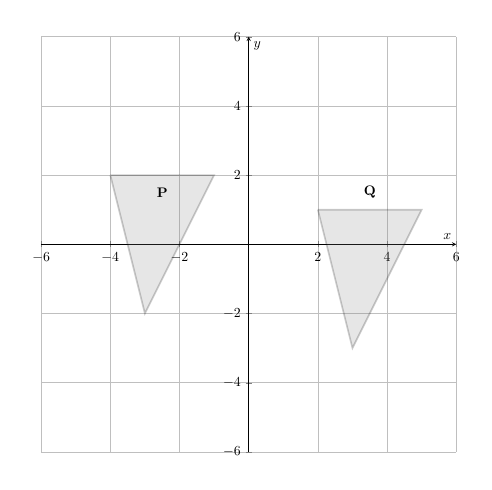
\begin{tikzpicture}[scale=0.5]
      \begin{axis}[
          xmin = -6, xmax = 6,
          ymin = -6, ymax = 6,
          grid = both,
          axis lines = middle,
          width = \textwidth,
          height = \textwidth,
          xlabel = {$x$},
          ylabel = {$y$},
        ]
        \filldraw[color=black, fill=gray, opacity=0.2, very thick] (-4,2) -- (-1,2) -- (-3,-2) -- (-4,2);
        \filldraw[color=black, fill=gray, opacity=0.2, very thick] (2,1) -- (5,1) -- (3,-3) -- (2,1);
        \node at (-2.5,1.5) {\textbf{P}};
        \node at (3.5,1.5) {\textbf{Q}};
      \end{axis}
    \end{tikzpicture}
  \end{figure}
  Describe fully the single transformation that maps triangle \textbf{P} onto triangle \textbf{Q}.\mrk{2}\\
  \tikz\draw[thick, dashed] (0,0) -- (0.9\textwidth,0);\\
  \tikz\draw[thick, dashed] (0,0) -- (0.9\textwidth,0);
  \item \mbox{}
  \begin{figure}[H]
    \centering
    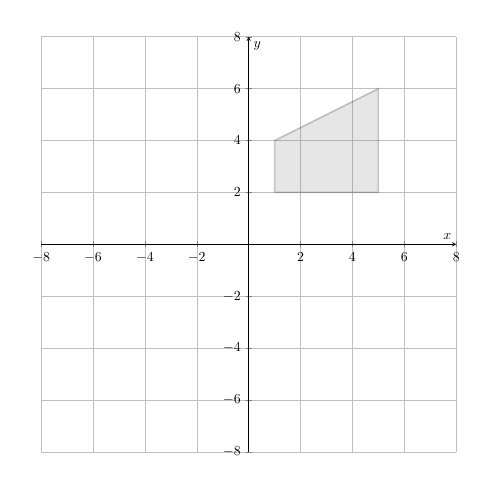
\begin{tikzpicture}[scale=0.5]
      \begin{axis}[
          xmin = -8, xmax = 8,
          ymin = -8, ymax = 8,
          grid = both,
          axis lines = middle,
          width = \textwidth,
          height = \textwidth,
          xlabel = {$x$},
          ylabel = {$y$},
      ]
      \filldraw[color=black, fill=gray, opacity=0.2, very thick] (1,2) -- (1,4) -- (5,6) -- (5,2) -- (1,2);
      \end{axis}
    \end{tikzpicture}
  \end{figure}
  Enlarge the shaded shape by scale factor $-\frac{1}{2}$ with centre $(-1, -2)$.\mrk{3}
  \item \mbox{}
  \begin{figure}[H]
    \centering
    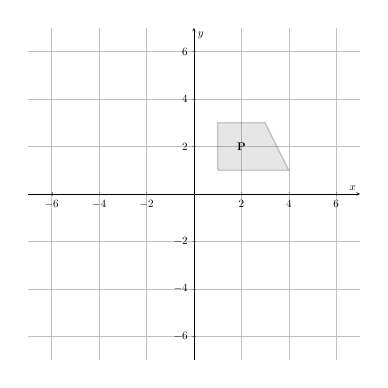
\begin{tikzpicture}[scale=0.4]
      \begin{axis}[
          xmin = -7, xmax = 7,
          ymin = -7, ymax = 7,
          grid = both,
          axis lines = middle,
          width = \textwidth,
          height = \textwidth,
          xlabel = {$x$},
          ylabel = {$y$},
        ]
        \filldraw[color=black, fill=gray, opacity=0.2, very thick] (1,1) -- (1,3) -- (3,3) -- (4,1) -- (1,1);
        \node at (2,2) {\textbf{P}};
      \end{axis}
    \end{tikzpicture}
  \end{figure}
  Shape $P$ is reflected in the line $x = -1$ to give shape $Q$.\\
  Shape $Q$ is reflected in the line $y = 0$ to give shape $R$.\\
  Describe fully the single transformation that maps shape $P$ onto shape $R$.\mrk{3}\\
  \tikz\draw[thick, dashed] (0,0) -- (0.9\textwidth,0);\\
  \tikz\draw[thick, dashed] (0,0) -- (0.9\textwidth,0);
  \item \mbox{}
  \begin{figure}[H]
    \centering
    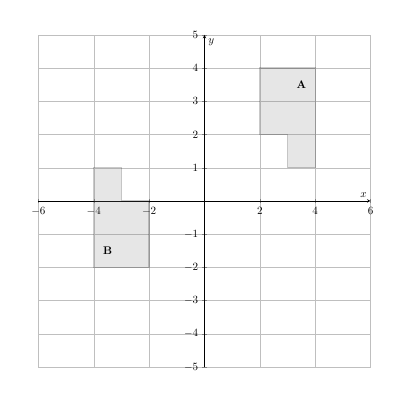
\begin{tikzpicture}[scale=0.4]
      \begin{axis}[
          xmin = -6, xmax = 6,
          ymin = -5, ymax = 5,
          grid = both,
          axis lines = middle,
          width = \textwidth,
          height = \textwidth,
          xlabel = {$x$},
          ylabel = {$y$},
        ]
        \filldraw[color=black, fill=gray, opacity=0.2, very thick]
          (3,1) -- (4,1) -- (4,4) -- (2,4) -- (2,2) -- (3,2) -- (3,1);

        \filldraw[color=black, fill=gray, opacity=0.2, very thick]
          (-3,1) -- (-4,1) -- (-4,-2) -- (-2,-2) -- (-2,0) -- (-3,0) -- cycle;

        \node at (3.5,3.5) {\textbf{A}};
        \node at (-3.5,-1.5) {\textbf{B}};
      \end{axis}
    \end{tikzpicture}
  \end{figure}
  Describe fully the single transformation that maps shape \textbf{A} onto shape \textbf{B}\mrk{3}\\
  \tikz\draw[thick, dashed] (0,0) -- (0.9\textwidth,0);\\
  \tikz\draw[thick, dashed] (0,0) -- (0.9\textwidth,0);
  \item \mbox{}
  \begin{figure}[H]
    \centering
    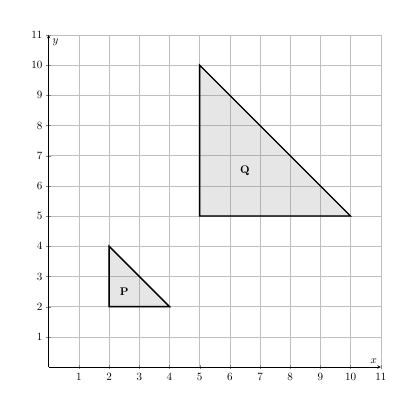
\begin{tikzpicture}[scale=0.4]
      \begin{axis}[
          xmin = 0, xmax = 11,
          ymin = 0, ymax = 11,
          grid = both,
          axis lines = middle,
          width = \textwidth,
          height = \textwidth,
          xlabel = {$x$},
          ylabel = {$y$},
        ]
        \filldraw[color=black, fill=gray, opacity=0.2, very thick]
          (2,2) -- (4,2) -- (2,4) -- cycle;
        \draw[color=black, very thick]
          (2,2) -- (4,2) -- (2,4) -- cycle;

        \filldraw[color=black, fill=gray, opacity=0.2, very thick]
          (5,5) -- (10,5) -- (5,10) -- cycle;
        \draw[color=black, very thick]
          (5,5) -- (10,5) -- (5,10) -- cycle;

        \node at (2.5,2.5) {\textbf{P}};
        \node at (6.5,6.5) {\textbf{Q}};
      \end{axis}
    \end{tikzpicture}
  \end{figure}
  Describe fully the single transformation that maps shape \textbf{P} onto shape \textbf{Q}.\mrk{3}\\
  \tikz\draw[thick, dashed] (0,0) -- (0.9\textwidth,0);\\
  \tikz\draw[thick, dashed] (0,0) -- (0.9\textwidth,0);
  \item \mbox{}
  \begin{figure}[H]
    \centering
    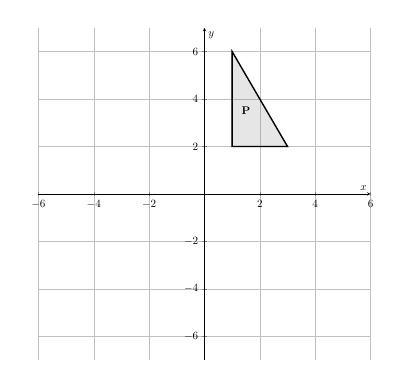
\begin{tikzpicture}[scale=0.4]
      \begin{axis}[
          xmin = -6, xmax = 6,
          ymin = -7, ymax = 7,
          grid = both,
          axis lines = middle,
          width = \textwidth,
          height = \textwidth,
          xlabel = {$x$},
          ylabel = {$y$},
        ]
        \filldraw[color=black, fill=gray, opacity=0.2, very thick]
          (1,2) -- (3,2) -- (1,6) -- cycle;
        \draw[color=black, very thick]
          (1,2) -- (3,2) -- (1,6) -- cycle;

        \node at (1.5,3.5) {\textbf{P}};
      \end{axis}
    \end{tikzpicture}
  \end{figure}
  Triangle \textbf{P} is drawn on a coordinate grid. The triangle \textbf{P} is reflected in the line $x = -1$ and then reflected in the line $y = 1$ to give triangle \textbf{Q}.\\
  Describe fully the single transformation which maps triangle \textbf{P} onto triangle \textbf{Q}.\mrk{3}\\
  \tikz\draw[thick, dashed] (0,0) -- (0.9\textwidth,0);\\
  \tikz\draw[thick, dashed] (0,0) -- (0.9\textwidth,0);
  \item \mbox{}
  \begin{figure}[H]
    \centering
    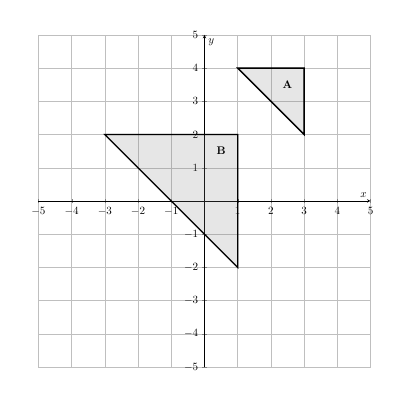
\begin{tikzpicture}[scale=0.4]
      \begin{axis}[
          xmin = -5, xmax = 5,
          ymin = -5, ymax = 5,
          grid = both,
          axis lines = middle,
          width = \textwidth,
          height = \textwidth,
          xlabel = {$x$},
          ylabel = {$y$},
        ]
        \filldraw[color=black, fill=gray, opacity=0.2, very thick]
          (1,4) -- (3,2) -- (3,4) -- cycle;
        \draw[color=black, very thick]
          (1,4) -- (3,2) -- (3,4) -- cycle;

        \filldraw[color=black, fill=gray, opacity=0.2, very thick]
          (-3,2) -- (1,2) -- (1,-2) -- cycle;
        \draw[color=black, very thick]
          (-3,2) -- (1,2) -- (1,-2) -- cycle;

        \node at (2.5,3.5) {\textbf{A}};
        \node at (0.5,1.5) {\textbf{B}};
      \end{axis}
    \end{tikzpicture}
  \end{figure}
  Triangle \textbf{A} and triangle \textbf{B} are drawn on the grid.
  \begin{enumerate}
    \item Describe fully the single transformation which maps triangle \textbf{A} onto triangle \textbf{B}.\mrk{3}\\
    \tikz\draw[thick, dashed] (0,0) -- (0.8\textwidth,0);\\
    \tikz\draw[thick, dashed] (0,0) -- (0.8\textwidth,0);
    \item \mbox{}
    \begin{figure}[H]
      \centering
      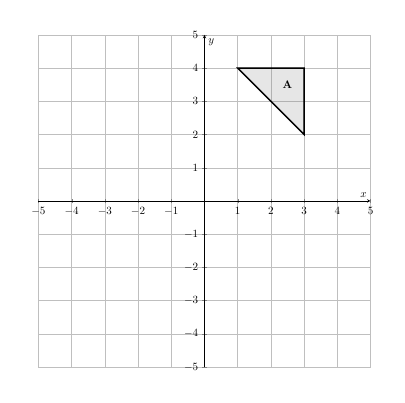
\begin{tikzpicture}[scale=0.4]
        \begin{axis}[
            xmin = -5, xmax = 5,
            ymin = -5, ymax = 5,
            grid = both,
            axis lines = middle,
            width = \textwidth,
            height = \textwidth,
            xlabel = {$x$},
            ylabel = {$y$},
          ]
          \filldraw[color=black, fill=gray, opacity=0.2, very thick]
            (1,4) -- (3,2) -- (3,4) -- cycle;
          \draw[color=black, very thick]
            (1,4) -- (3,2) -- (3,4) -- cycle;
  
          \node at (2.5,3.5) {\textbf{A}};
        \end{axis}
      \end{tikzpicture}
    \end{figure}
    Reflect triangle \textbf{A} in the line $x = 4$.\mrk{2}
  \end{enumerate}
  \newpage
  \item %
  \begin{enumerate}
    \item \mbox{}
    \begin{figure}[H]
      \centering
      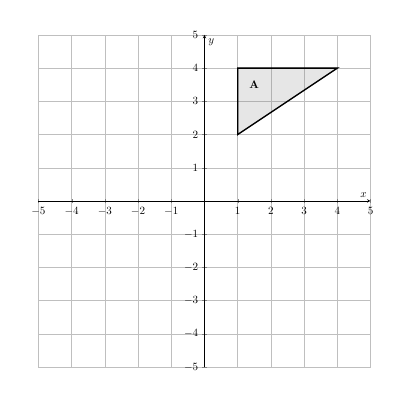
\begin{tikzpicture}[scale=0.4]
        \begin{axis}[
            xmin = -5, xmax = 5,
            ymin = -5, ymax = 5,
            grid = both,
            axis lines = middle,
            width = \textwidth,
            height = \textwidth,
            xlabel = {$x$},
            ylabel = {$y$},
          ]
          \filldraw[color=black, fill=gray, opacity=0.2, very thick]
            (1,2) -- (1,4) -- (4,4) -- cycle;
          \draw[color=black, very thick]
            (1,2) -- (1,4) -- (4,4) -- cycle;
  
          \node at (1.5,3.5) {\textbf{A}};
        \end{axis}
      \end{tikzpicture}
    \end{figure}
    Rotate triangle $A$ $\ang{90}$ clockwise, centre $O$.
    \item \mbox{}
    \begin{figure}[H]
      \centering
      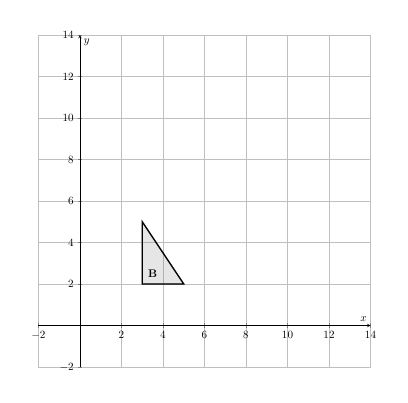
\begin{tikzpicture}[scale=0.4]
        \begin{axis}[
            xmin = -2, xmax = 14,
            ymin = -2, ymax = 14,
            grid = both,
            axis lines = middle,
            width = \textwidth,
            height = \textwidth,
            xlabel = {$x$},
            ylabel = {$y$},
          ]
          \filldraw[color=black, fill=gray, opacity=0.2, very thick]
            (3,2) -- (5,2) -- (3,5) -- cycle;
          \draw[color=black, very thick]
            (3,2) -- (5,2) -- (3,5) -- cycle;
  
          \node at (3.5,2.5) {\textbf{B}};
        \end{axis}
      \end{tikzpicture}
    \end{figure}
    Enlarge triangle \textbf{B} by scale factor $3$, centre $(1, 2)$.
  \end{enumerate}



\end{enumerate}